\documentclass[11pt,a4paper]{article}

\usepackage[utf8]{inputenc}
\usepackage[greek,english]{babel}
\usepackage{alphabeta} 

\usepackage[pdftex]{graphicx}
\usepackage[top=1in, bottom=1in, left=1in, right=1in]{geometry}

\linespread{1.06}
\setlength{\parskip}{8pt plus2pt minus2pt}

\widowpenalty 10000
\clubpenalty 10000

\newcommand{\eat}[1]{}
\newcommand{\HRule}{\rule{\linewidth}{0.5mm}}

\usepackage[official]{eurosym}
\usepackage{enumitem}
\setlist{nolistsep,noitemsep}
\usepackage[hidelinks]{hyperref}
\usepackage{cite}
\usepackage{lipsum}
\graphicspath{ {/home/anon/Pictures/} }


\begin{document}

%===========================================================
\begin{titlepage}
\begin{center}

% Top 

% Title
\HRule \\[0.4cm]
{ 
Spring Semester 2020-2021\\[0.2cm]
\large{\bf A Report for CSN-361 (Computer Networks Lab)}\\[0.4cm]
}
\HRule \\[1.5cm]

Submitted by\\[0.5cm]
% Author
{
{\bf Masih Ahmed (18117056)}\\[0.1cm]
\texttt{mahmed@cs.iitr.ac.in}\\[0.1cm]
}

\vfill

\includegraphics[width=0.3\textwidth]{IITR_new_logo_color.jpg}~\\[0.5cm]
\textsc{\large Department of Computer Science and Engineering}\\[0.2cm]
\textsc{\large Indian Institute of Technology (IIT) Roorkee}\\[0.2cm]

% Bottom
{\large \today}
 
\end{center}
\end{titlepage}

\addtocontents{toc}{\protect\thispagestyle{empty}}

\newpage

%===========================================================
\tableofcontents
\addtocontents{toc}{\protect\thispagestyle{empty}}
\newpage
\setcounter{page}{1}
%===========================================================

%===========================================================
\section{Problem Statement 1}\label{sec:problem1}
%===========================================================
\subsection{Question}\label{sec:question1}
Write a C++ program to print the MAC address of your computer, the host name and the IP address of your
computer.

\subsection{Theory}\label{sec:theory1}
A media access control address (MAC address) is a unique 48-bit/64-bit value assigned to a network interface controller (NIC) for use as a network address in communications within a network segment.

An IP address is a unique 32-bit/128-bit address that identifies a device on the internet or a local network.

A hostname is a unique name for a computer or network node in a network. Hostnames are specific names or character strings that refer to a host and make it usable for the network and people.

\subsection{Implementation Details}\label{sec:details1}
The MAC address can be retrieved in Linux by reading the file from /sys/class/net/eno1/address for the ethernet NIC and /sys/class/net/wlo1/address for the wireless NIC.

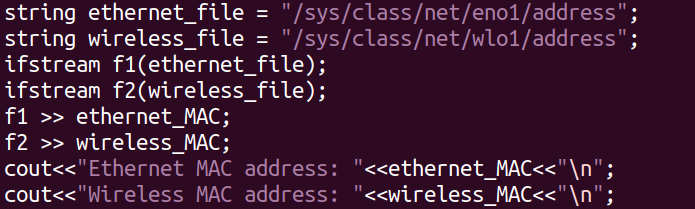
\includegraphics[width=1\textwidth]{p1_mac.png}

The hostname and IP can be found out using the gethostname() and gethostbyname() functions. gethostbyname() returns a structure containing all relevant host details, from which IP can be found out.

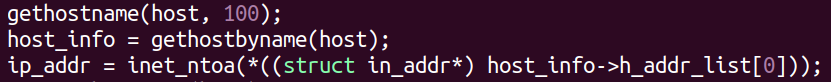
\includegraphics[width=0.7\textwidth]{p1_ip_hostname.png}


\subsection{Results}\label{sec:results1}
The relevant MAC addresses, hostname and IP addresses are printed.

\includegraphics[width=0.5\textwidth]p1_res.png}


%===========================================================
\section{Problem Statement 2}\label{sec:problem2}
%===========================================================
\subsection{Question}\label{sec:question2}
Write a socket program in Java for PING command.

\subsection{Theory}\label{sec:theory2}
Ping is a command-line utility that acts as a test to see if a networked device is reachable.

The ping command sends an ICMP echo request over the network to a specific device. A successful ping results in an ICMP echo reply from the computer that was pinged back to the originating computer. The time elapsed\textit{ (Round trip time)} is measured and is reported as ping.

Ping uses ICMP and sends echo packets to the host which sends and ICMP reply message back if it is available.

\subsection{Implementation Details}\label{sec:details2}
Java doesn't support ICMP, hence raw sockets can't be created. But a class called \emph{InetAddress} has a function named \textit{isReachable} which is used to check if an address is reachable within a certain time limit. When run with suitable privileges, it emulates the ping command and is able to send ICMP packets. 


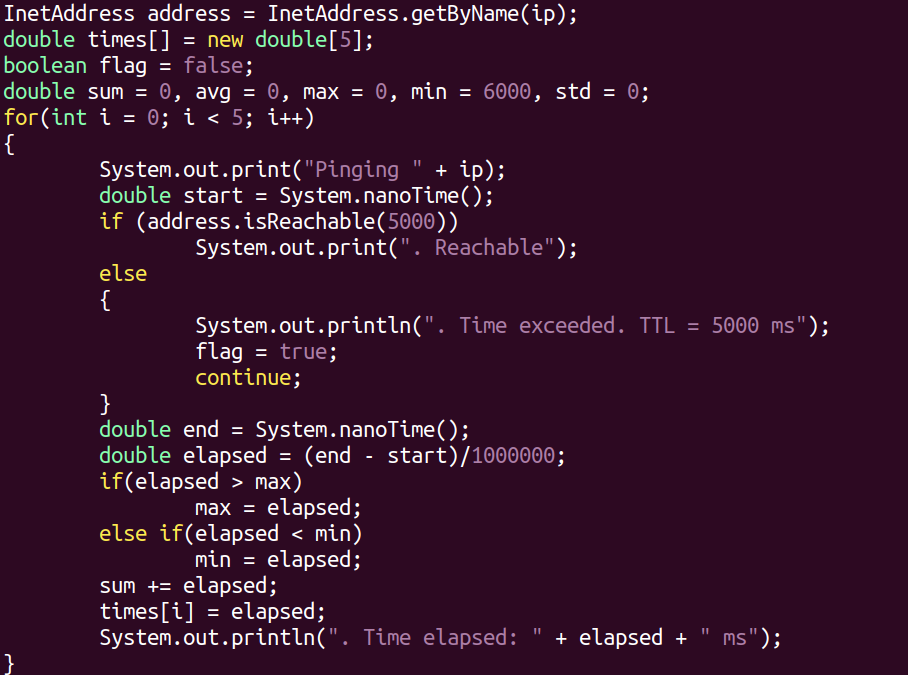
\includegraphics[width=0.7\textwidth]{p2_inet.png}


\subsection{Results}\label{sec:results2}
Th

\includegraphics[width=1\textwidth]{p2_res}


%===========================================================
\section{Problem Statement 3}\label{sec:problem3}
%===========================================================
\subsection{Question}\label{sec:question3}
Implement an error detection mechanism using the standard CRC algorithm. Write two programs: generator and verifier. The generator program reads from standard input an n-bit message as a string of 0’s and 1’s as a line of ASCII text. The second line is the k-bit polynomial, also in ASCII. It first checks that the polynomial is not divisible by x and x+1. If it is divisible by x or x+1, it outputs error else it outputs to standard output a line of ASCII text with n+k-1 0’s and 1’s representing the message to be transmitted. Then it outputs the polynomial, just as it read it in. The verifier program reads in the output of the generator program (if output is not error) and outputs a message indicating whether it is correct or not. Finally write a program, alter, that inverts one bit in the first line of the output of the generator depending on its argument, but copies rest of the first line and second line correctly. Now type the following and report the outcome.
(i) generator < file | verifier
(ii) generator < file | alter arg | verifier

\subsection{Theory}\label{sec:theory3}
Cyclic Redundancy Check (CRC) is a block code used to detect accidental changes to raw data transmitted via digital networks and storage devices.

CRC involves binary division of the data bits being sent by a predetermined divisor agreed upon by both the communicating parties. The divisor is generated using polynomials.
Blocks of data entering these systems get a short check value attached, based on the remainder of a polynomial division of their contents. On retrieval, the calculation is repeated and, in the event the check values do not match, corrective action can be taken against data corruption.

When messages are encoded using CRC, a fixed polynomial called generator polynomial,G(x) is used. The value of is mutually agreed upon by the sending and the receiving parties. A k – bit word is represented by a polynomial which ranges from X0 to xk-1. The order of this polynomial is the power of the highest coefficient, i.e.(K-1) The length of G(x) should be less than the length of the message it encodes. Also, both its MSB and LSB should be 1. In the process of encoding, CRC bits are appended to the message so that the resultant frame is divisible by G(x).

\textbf{Algorithm for Encoding using CRC}

\begin{itemize}

\item The communicating parties agree upon the size of message,M(x) and the generator polynomial, G(x).

\item If r is the order of G(x),r, bits are appended to the low order end of M(x) to obtain the block.

\item The block is divided by G(x) using modulo 2 division.

\item The remainder after division is added to the block using modulo 2 addition. The result is the frame to be transmitted, T(x). The encoding procedure makes T(x) exactly divisible by G(x).

\end{itemize}

\textbf{Algorithm for Decoding using CRC}

\begin{itemize}

\item The receiver divides the incoming data frame T(x) unit by G(x) using modulo 2 division. Mathematically, if E(x) is the error, then modulo 2 division of [M(x) + E(x)] by G(x) is done.

\item If the remainder is zero, then it implies that E(x) is zero i.e. there are no errors. The data frame is accepted.

\item A non-zero remainder indicates a non-zero value of E(x), or in other words presence of an error. So the data frame is rejected. The receiver may then send an erroneous acknowledgment back to the sender for retransmission.

\end{itemize}

\subsection{Implementation Details}\label{sec:details3}
As the question states, we take the input and first check whether the polynomial is divisible by x or x+1.
If it turns out to be divisible by either of the two, error is shown and the program terminates.

\includegraphics[width=1\textwidth]{impl_3_1}

If the polynomial is not divisible by both x and x+1, the message is encoded using the CRC encoding algorithm. The encoded message and the polynomial are printed as output.

\includegraphics[width=1\textwidth]{impl_3_2}

\includegraphics[width=1\textwidth]{impl_3_3}
The verifier runs the CRC decoding algorithm on the output message by the generator. If the generator outputs "Error", no computation is done.


\subsection{Results}\label{sec:results3}
For the input : 

\includegraphics[width=0.3\textwidth]{res_3_1}

We see the outputs as : 

\includegraphics[width=0.9\textwidth]{res_3_4}

\includegraphics[width=1\textwidth]{res_3_2}

\includegraphics[width=1\textwidth]{res_3_3}

%===========================================================
\section{Problem Statement 4}\label{sec:problem4}
%===========================================================
\subsection{Question}\label{sec:question4}
Write a C++/Java program that accepts an IP address and subnet mask in CIDR notation, and print the following information about the sub-network:
1) Subnet Mask in dotted decimal notation (Example 255.0.0.0)
2) Network Address in dotted decimal notation: (Example 103.0.0.0)
3) Usable Host IP Range: Starting IP 103.0.0.1 --- Ending IP 103.255.255.254

\subsection{Theory}\label{sec:theory4}
CIDR notation is a compact representation of an IP address and its associated network mask. CIDR notation specifies an IP address, a slash ('/') character, and a decimal number. The decimal number is the count of leading 1 bits in the network mask. The number can also be thought of as the width (in bits) of the network prefix. The IP address in CIDR notation is always represented according to the standards for IPv4 or IPv6.

The subnet mask splits the IP address into the host and network addresses, thereby defining which part of the IP address belongs to the device and which part belongs to the network.

\subsection{Implementation Details}\label{sec:details4}
We take as input the IP address (IPv4) in CIDR notation and parse the input into the IP and the mask.

The subnet mask is calculated using the parsed integer mask value :

\includegraphics[width=1\textwidth]{impl_4_1}

Next, using the input IP and the subnet mask, the Network Address is calculated. The first and last IP addresses of the network are then calculated using the Network Address.

\includegraphics[width=1\textwidth]{impl_4_2}

\subsection{Results}\label{sec:results4}
We have the outputs for the following test cases as:
\begin{itemize}
    \item 103.67.20.12/8
    
    \includegraphics[width=0.75\textwidth]{res_4_1}
    
    \item 172.45.3.19/23
    
    \includegraphics[width=0.75\textwidth]{res_4_2}
    
\end{itemize}

%===========================================================
\section{Problem Statement 5}\label{sec:problem5}
%===========================================================
\subsection{Question}\label{sec:question5}
Write a program that an instructor can use to demonstrate the method of calculating IPv4 checksum. Your program should ask the user to enter the values of different fields of an IPv4 header. It should then calculate IPv4 checksum. Your program should not only show the final result but should also demonstrate the method (each step) to calculate the checksum.

\subsection{Theory}\label{sec:theory5}
The IPv4 header checksum is a checksum used in version 4 of the Internet Protocol (IPv4) to detect corruption in the header of IPv4 packets. It is carried in the IP packet header, and represents the 16-bit result of summation of the header words.[1]

The checksum calculation is defined in RFC 791:[3]

\emph{The checksum field is the 16-bit ones' complement of the ones' complement sum of all 16-bit words in the header. For purposes of computing the checksum, the value of the checksum field is zero.}

If there is no corruption, the result of summing the entire IP header, including checksum, should be zero. At each hop, the checksum is verified. Packets with checksum mismatch are discarded. The router must adjust the checksum if it changes the IP header

\subsection{Implementation Details}\label{sec:details5}

We take input of all fields of the IPv4 header from the user. The fields are grouped to form 16 bit words. These 16-bit words are summed up and any carry over is also added to the numbers to obtain the final sum.

\includegraphics[width=0.75\textwidth]{impl_5_1}

Finally, we take one's complement of the final sum to obtain the checksum.

\includegraphics[width=0.75\textwidth]{impl_5_2}

\subsection{Results}\label{sec:results5}
We have the results for the following testcases:
\begin{itemize}
    \item 4500 003c 1c46 4000 4006 0000 ac10 0a63 ac10 0a0c
    
    \includegraphics[width=0.7\textwidth]{res_5_1}
    
    \hspace{1 pt}
    
    \item a500 0040 1bbc 400c 0806 0000 ac0c 1008 ac10 0c11 abcd
    
    \includegraphics[width=0.7\textwidth]{res_5_2}
    
\end{itemize}

%===========================================================
\section{Problem Statement 6}\label{sec:problem6}
%===========================================================
\subsection{Question}\label{sec:question6}
Write a C++/Java program for the Decibel (dB) calculator. You program should perform the following operations:
1) If transmit power of a network device is given in watts (Example: ‘20 W’) then the program should print the transmit power in Decibel Watts (dBW) and Decibel Milliwatts (dBm).
2) Else if transmit power of a network device is given in Decibel Watts (dBW) or Decibel Milliwatts (Example: ‘20 dBW’ or ‘20 dBm’) then the program should print the transmit power in Watts.

\subsection{Theory}\label{sec:theory6}
The power P(dBm) in dBm is equal to 10 times the base 10 logarithm of 1000 times the power P(W) in watts (W) divided by 1 watt (W)

dBW or decibel-watt is a unit of power in decibel scale, referenced to 1 watt (W).
The power in decibel-watts (P(dBW)) is equal to 10 times base 10 logarithm of the power in watts (P(W))

\subsection{Implementation Details}\label{sec:details6}
Input is taken from the user and the units are detected:

\includegraphics[width=0.7\textwidth]{impl_6_1}

\hspace{1 pt}

Finally the appropriate conversion is done:

\includegraphics[width=0.6\textwidth]{impl_6_2}

\subsection{Results}\label{sec:results6}
The following outputs can be seen for the testcases: 

\includegraphics[width=0.5\textwidth]{res_6_1}

\includegraphics[width=0.5\textwidth]{res_6_2}

\includegraphics[width=0.5\textwidth]{res_6_3}

\end{document} 
